%!TEX root = ../crimson_throne_book_main.tex
% 2016-07-02
The stairs lead to the bowels of the crypts below the temple of Asmodeus.\hyperref[fig:Akaruzug-for-blood-clone-production-619036747]{ A strange construct floats in the center of a burning five-pointed star. } The grim statue quietly hovers, its slow, seemingly weightless bobbing belying its obvious bulk. Sculpted in the shape of a grim, horned angel, gigantic wings and terrible, long clawed arms jut from a legless body that tapers into a blunt, blade-like trunk. Crucified upon the ominous form's breast hangs the drained body of Cressida Kroft, Korvosa's field marshal. Five large vats stand in the points of the star; blood drips from the ceiling into these container. The crimson fluid churns and bubbles as it is slowly molded into human shape. The sanguine women are in different stages of development, with the most advanced specimen trying to tear loose from the scarlet goo. Off to the right is archbishop Ornher Reebs, the temple's high priest, and his bodyguard Mallas. \\

\begin{figure}[h]
	\centering
	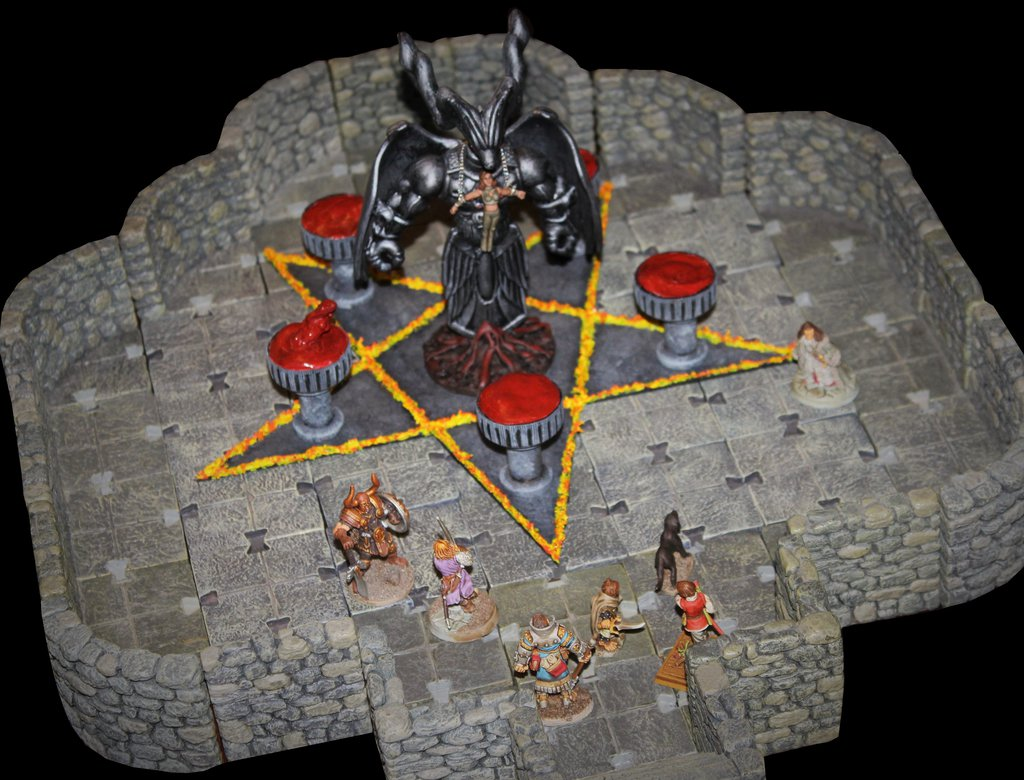
\includegraphics[width=0.4\textwidth]{images/Akaruzug-for-blood-clone-production-619036747_mod.jpg}
	\caption{Akaruzug for blood clone production}
	\label{fig:Akaruzug-for-blood-clone-production-619036747}
\end{figure}

Quint still poses as an inquisitor of Asmodeus and forcefully orders Reebs to cease these bestialities immediately, as they go against Korvosan rule. Reebs is not fazed in the least by this display of jurisdiction, he is not opposing the law, as a matter of fact, he's acting on behalf of the city's highest authority, the queen herself. On top of that his practice, albeit somewhat unusual, fits perfectly in Asmodean doctrine: sacrifices for the greater good and promotion of Asmodeus' devil kingdom. In vain Quint tries to contest Reebs's claims, but the high priest simply calls out to his god: {\itshape``Asmodeus, show us who is right here!}'' His bodyguard takes this as a clue to draw his sword, but the real response to the archbishop's calling is given within the burning star:\hyperref[fig:Akaruzug-in-Curse-of-the-Crimson-Throne-619030501]{ with a sudden jut the humongous statue snaps to life and two of the vats burst out into horrible humanoid shapes that ooze and weep blood from every part of their body; their hands end in sharpened claws. }  \\

\begin{figure}[h]
	\centering
	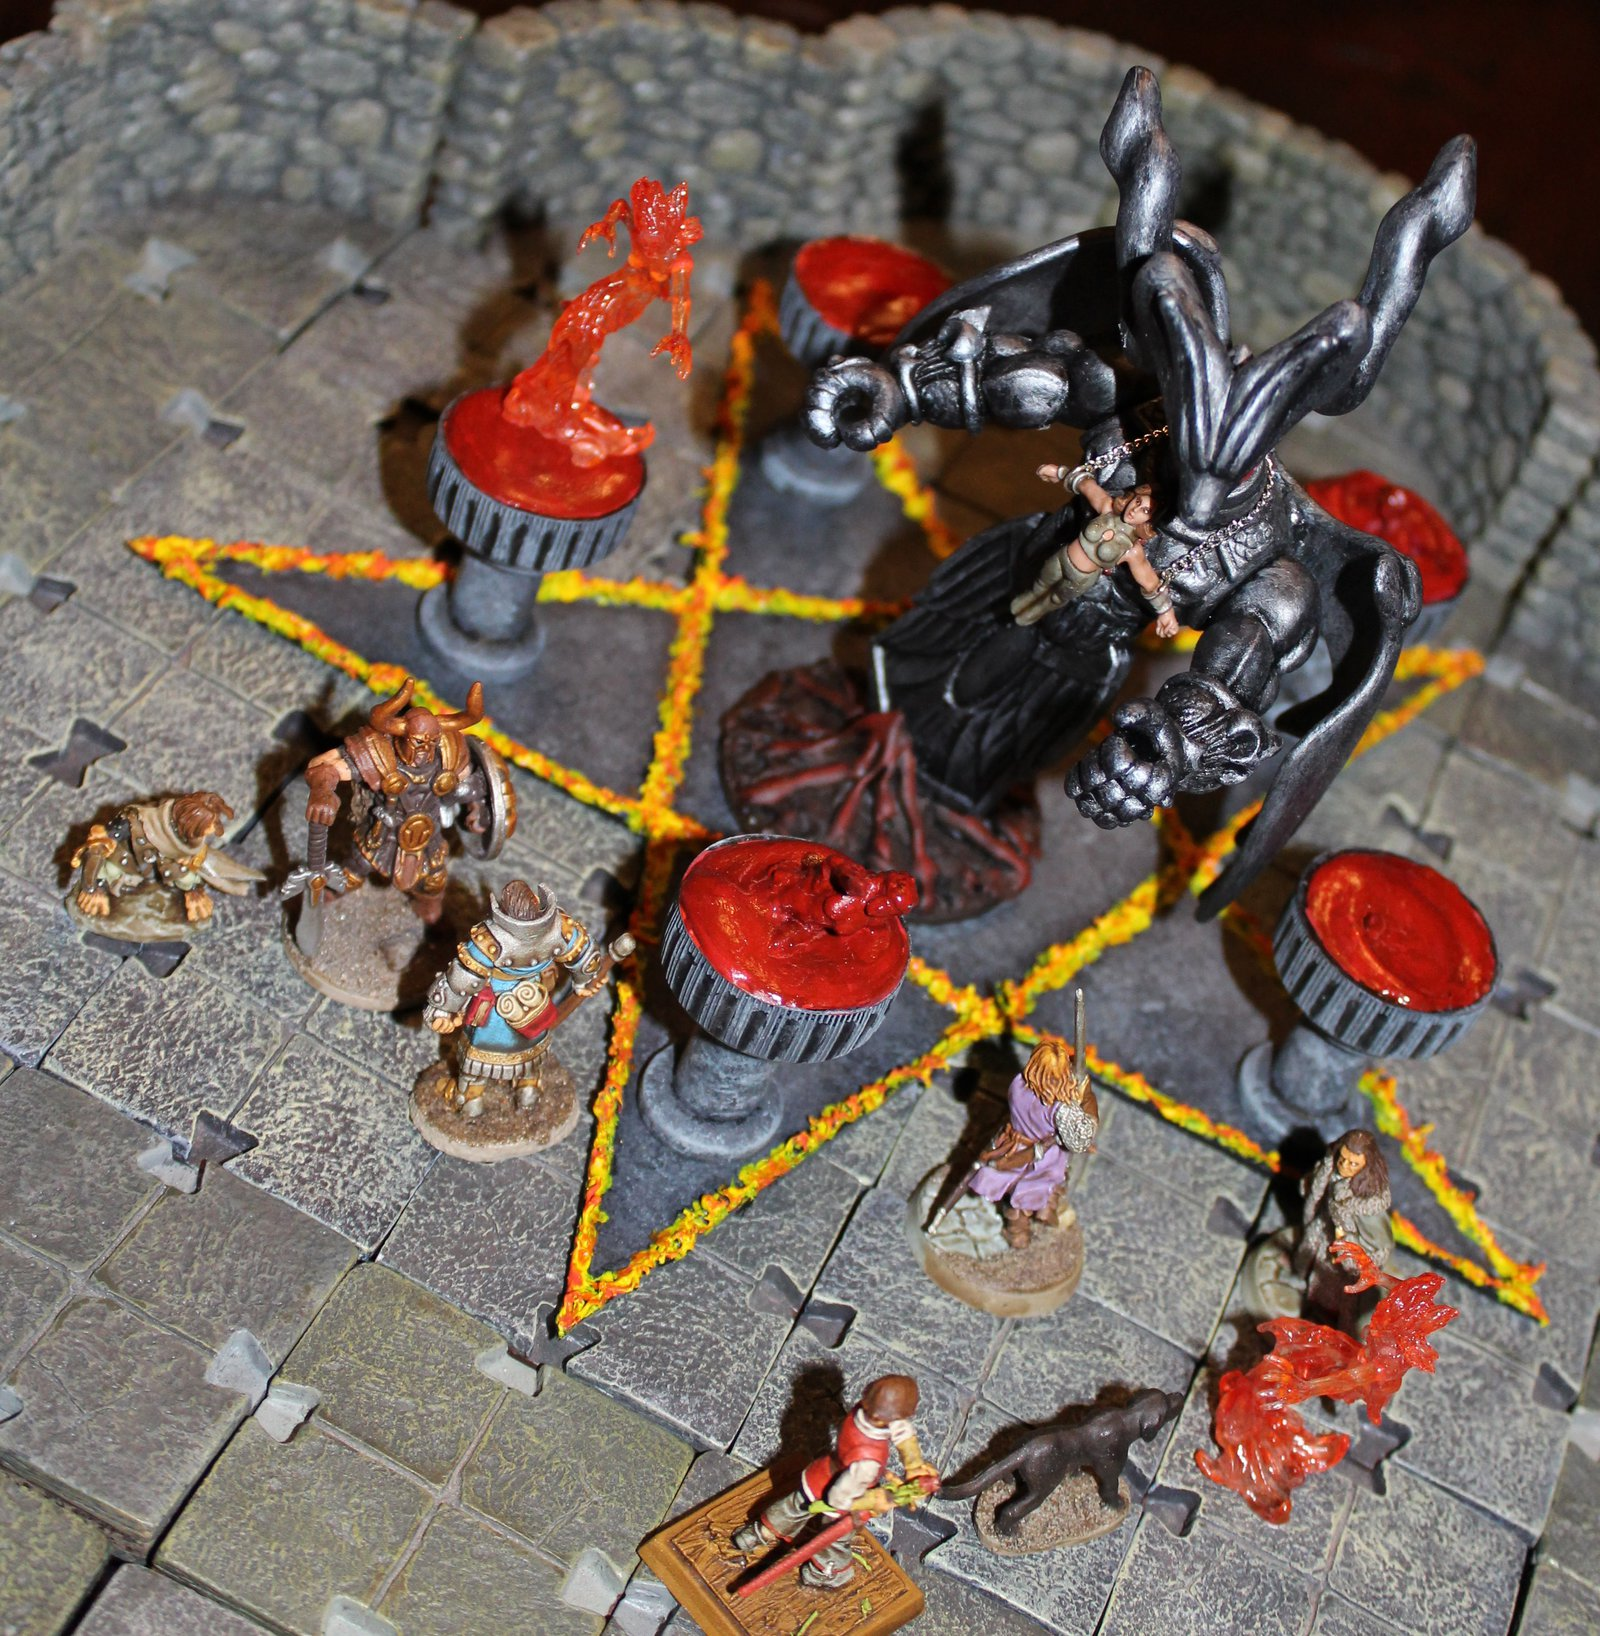
\includegraphics[width=0.4\textwidth]{images/Akaruzug-in-Curse-of-the-Crimson-Throne-619030501_mod.jpg}
	\caption{Akaruzug in Curse of the Crimson Throne}
	\label{fig:Akaruzug-in-Curse-of-the-Crimson-Throne-619030501}
\end{figure}

These fresh blood wights are the first to act, charging Balian and Quint. Vencarlo tries to counter, but finds that his rapier has difficulty piercing the creatures' viscous skin. Reebs calls a wall of swirling blades into existence on top of Vencarlo, Balian and Quint, cleverly cutting off Spyder, Puk and Sjo from the rest of the room. Fortunately the three heroes in the {\itshape blade barrier} manage to jump out of harm's way. Puk tumbles forward through the wall, relying on his roguish skills to avoid the hacking swords, and focuses his attacks on the same blood wight that Balian is targeting. Next the akaruzug flies closer, wipping its bladed underbody at Quint. The bard makes a converse movement and steps back to look for cover on the other side of the  {\itshape blade barrier} . He suffers some cuts, but now finds himself in a relatively safe position to cast spells and try to influence the battle. He boosts his friends with  {\itshape haste} and starts his  {\itshape satire} to debuff his enemies, using the infernal language to do so. It looks like his effort fails on the construct and on Mallas as well, who is probably too stupid to know the tongue of his patron deity. Sjo attempts to  {\itshape hold} the broad-shouldered bodyguard in place, but the temple warrior withstands the magic. Spyder joins the fight on the other side of the  {\itshape barrier} , but suffers the full strength of the blades while jumping through. The poor dog is badly hurt and its bad luck continues as both the akaruzug and Mallas bear down on it in full force. Mangled and bleeding from many wounds the canine drops to the floor. Ornher Reebs calls down a large pillar of fire on the center of combat, catching most heroes and the two blood wights in the flames. One of the latter does not survive the fire. The heroes now press the attack on its sibling, but the akaruzug claws and slashes its way through them without mercy, taking Puk down as well. Sjo heals his friends with a  {\itshape mass cure light wounds} and calls down his own  {\itshape flame strike} on Mallas and Reebs. At the same time Quint casts  {\itshape good hope} and drops his  {\itshape satire} in favor of  {\itshape inspire greatness} for Balian and Puk. The halfling's luck picks up as he slips under Mallas's fierce swing and Balian shares in the good fortune when his armor protects him from the blood wight's claws. Vencarlo finally manages to finish the wight off, but still finds himself and his allies cornered by the hovering akaruzug. Puk uses his cloak's  {\itshape dimension door} power to teleport himself, Balian and Vencarlo to the other side of the room, next to Reebs. The high priest has just enough time to summon a look of surprise and panic on his face, before the halfing's daggers and Balian's greatsword end his miserable existence. Sjo now manages to freeze Mallas in place with a  {\itshape hold person} , but just for a few seconds. Vencarlo darts around the floating construct, taking an attack of opportunity 'for the team', so he can provide flanking to Puk on Mallas. The fencing master gets hit even more by the akaruzug, but the seasoned warrior is tough and makes his stand. Mallas is not so lucky; when Puk and Balian charge him, he does not survive. Now the companions can at last focus on the flying statue. Quint uses his new {\itshape dimension door} spell to zap Sjo and himself to the other side of the  {\itshape blade barrier} , where the healer can finally restore Puk's faltering health. When the heroes deliver their first blows to the akaruzug, they notice that Cressida Kroft's crucified body seems to share in the agony of the wounds. Balian activates his  {\itshape boots of flying} to take to the air and cleaves through the chain that binds the field marshal to the construct's chest. His attempt succeeds and has an unexpected bonus. As the commander of the Korvosan Guard tumbles to the floor, the floating monstrosity suddenly freezes to a halt, giving the champions of Korvosa the opportunity to finish it off. Sjo heals the ailing field marshal and nurses her back to consciousness, although she still feels weak and hollow. The companions take a few moments to recover from the fight, gather some loot and brief Kroft. Then they head back to the floor with the cell block and free the imprisoned girls. After they reveal their true identity, some of the girls recognize them and realize they have indeed been saved. One of the prisoners is Aurelia Bromathan, niece to the leader of the rebellion, Illrem Bromathan. She is in a separate cell with eight other girls who look like they have been in here longer than the others. It turns out that they were considered 'impure sacrifices', as they have all given birth. (This confirms older rumors that Aurelia Bromathan, who disappeared from the city for a year, was indeed pregnant and shipped off to give birth the her 'bastard' in secret.) Quint convinces the girls to put on Gray Maiden armors, which are readily available in a well-stocked armory, so they can move through the city in disguise. He has no problem leading them past the guards at the front temple gate and after a quick stop at the old courthouse to pick up Keppira d'Bear, they make their way back to the Gray District. Using Puk, Balian and Vencarlo as scouts, the troop manages to avoid real Gray Maiden patrols and makes it to the other side of the city safely. When the finally reach the halls of the resistance, the companions get some much needed rest.\\

\section{26 Arodus 4708}

By the time the party gets up it is already past noon. Illrem calls the heroes into his makeshift office to thank them for rescuing his niece and get a full report on their rescue mission. When he learns about the infernal contract that Ileosa supposedly closed in the Acadamae, he is very worried. It seems that the queen has garnered even more superpower than the crown gives her. The leader of the resistance feels that this intel certainly deserves more attention. He summons Keppira d'Bear from the temple of Pharasma to shed some light on these diabolical dealings. The archbishop's knowledge is limited, though. She knows that such deals are usually forged by contract devil, also known as Phistophili. Apart from taking care of hell's bureaucracy, these devils seduce desperate, arrogant or foolish mortals to make a deal with Hell itself. Infernal contracts can provide several boons, but to gain those the mortal has to sign over his soul, dooming himself to eternal damnation after his death.\\

While numerous types of infernal contracts exist, the following three are those most often offered to mortals:\\

 